%%%%%%%%%%%%%%%%%%%%%%%%%%%%%%%%%%%%%%%%%
% Beamer Presentation
% LaTeX Template
% Version 1.0 (10/11/12)
%
% This template has been downloaded from:
% http://www.LaTeXTemplates.com
%
% License:
% CC BY-NC-SA 3.0 (http://creativecommons.org/licenses/by-nc-sa/3.0/)
%
%%%%%%%%%%%%%%%%%%%%%%%%%%%%%%%%%%%%%%%%%

%----------------------------------------------------------------------------------------
%	PACKAGES AND THEMES
%----------------------------------------------------------------------------------------

\documentclass{beamer}

\mode<presentation> {

% The Beamer class comes with a number of default slide themes
% which change the colors and layouts of slides. Below this is a list
% of all the themes, uncomment each in turn to see what they look like.

%\usetheme{default}
\usetheme{AnnArbor}
%\usetheme{Antibes}
%\usetheme{Bergen}
%\usetheme{Berkeley}
%\usetheme{Berlin}
%\usetheme{Boadilla}
%\usetheme{CambridgeUS}
%\usetheme{Copenhagen}
%\usetheme{Darmstadt}
%\usetheme{Dresden}
%\usetheme{Frankfurt}
%\usetheme{Goettingen}
%\usetheme{Hannover}
%\usetheme{Ilmenau}
%\usetheme{JuanLesPins}
%\usetheme{Luebeck}
%\usetheme{Madrid}
%\usetheme{Malmoe}
%\usetheme{Marburg}
%\usetheme{Montpellier}
%\usetheme{PaloAlto}
%\usetheme{Pittsburgh}
%\usetheme{Rochester}
%\usetheme{Singapore}
%\usetheme{Szeged}
%\usetheme{Warsaw}

% As well as themes, the Beamer class has a number of color themes
% for any slide theme. Uncomment each of these in turn to see how it
% changes the colors of your current slide theme.

%\usecolortheme{albatross}
%\usecolortheme{beaver}
%\usecolortheme{beetle}
%\usecolortheme{crane}
\usecolortheme{dolphin}
%\usecolortheme{dove}
%\usecolortheme{fly}
%\usecolortheme{lily}
%\usecolortheme{orchid}
%\usecolortheme{rose}
%\usecolortheme{seagull}
%\usecolortheme{seahorse}
%\usecolortheme{whale}
%\usecolortheme{wolverine}

%\setbeamertemplate{footline} % To remove the footer line in all slides uncomment this line
%\setbeamertemplate{footline}[page number] % To replace the footer line in all slides with a simple slide count uncomment this line

%\setbeamertemplate{navigation symbols}{} % To remove the navigation symbols from the bottom of all slides uncomment this line
}

\usepackage{graphicx} % Allows including images
\usepackage{booktabs} % Allows the use of \toprule, \midrule and \bottomrule in tables
\usepackage{subcaption}

%----------------------------------------------------------------------------------------
%	TITLE PAGE
%----------------------------------------------------------------------------------------

\title[RCS]{Electromagnetic Simulations in FEKO} % The short title appears at the bottom of every slide, the full title is only on the title page

\author{Vikas Kurapati} % Your name
\institute[IITB] % Your institution as it will appear on the bottom of every slide, may be shorthand to save space
{
Department of Aerospace Engineering \\ % Your institution for the title page
\medskip
\textrm{IIT Bombay} % Your email address
}
\date{\today} % Date, can be changed to a custom date

\begin{document}

\begin{frame}
\titlepage % Print the title page as the first slide
\end{frame}

\begin{frame}
\frametitle{Overview} % Table of contents slide, comment this block out to remove it
\tableofcontents % Throughout your presentation, if you choose to use \section{} and \subsection{} commands, these will automatically be printed on this slide as an overview of your presentation
\end{frame}

%----------------------------------------------------------------------------------------
%	PRESENTATION SLIDES
%----------------------------------------------------------------------------------------
\begin{frame}
\section{Theory}
\frametitle{Theory}
In performing electromagnetic simulations to be shown in the upcoming slides, FEKO software was used. FEKO software uses different schemes of which Method of Moments(MOM), Multilevel Fast Multipole Method(MLFMM), Physical Optics(PO) schemes were used as and when required according to the frequency of the problem being simulated.
\end{frame}

\begin{frame}
\frametitle{Theory}
\subsection{Definition of RCS}
\textbf{RCS}: RCS(Radar Cross section is defined as a measure of reflective strength of a target defined as $4\pi$ times the ratio of the power per unit solid angle scattered  in a specified direction to the power per unit area in a plane wave incident on the scatterer from a specified direction. More precisely it is the limit of that ratio as the distance from the scatterer to the point where the scattered power is measure approaches infinity:
\begin{equation}
\sigma = \lim_{r\to\infty} 4\pi r^2 \frac{|\textbf{E}^{scat}|^2}{|\textbf{E}^{inc}|^2}
\end{equation}
Due to large dynamic range of RCS, a logarithmic power scale is most often used with the reference value of $\sigma_{ref} = 1 m^2$:
\begin{equation}
\sigma_{dBsm} = \sigma_{dBm^2} = 10log_{10}(\frac{\sigma_{m^2}}{\sigma_{ref}}) = 10log_{10}(\frac{\sigma_{m^2}}{1})
\end{equation}
\end{frame}
\begin{frame}
\frametitle{Theory}
To find RCS of a particular body under a particular illumination, we need to solve Maxwell's equations and find the scattered portion of the illumination.\\
The electromagnetic integral equations were obtained by Stratton Chu using the vector Green's Theorem in conjunction with Maxwell's equations. The total electric and magnetic fields are written as the sum of the incident and scattered fields:
\begin{eqnarray}
\textbf{E}^T = \textbf{E}^i + \textbf{E}^s \\
\textbf{H}^T = \textbf{H}^i + \textbf{H}^s
\end{eqnarray}
\end{frame}

\begin{frame}
\frametitle{Theory}
The scattered \textbf{E} and \textbf{H} are given by Stratton-Chu integrals:
\begin{eqnarray}
\textbf{E}^s = \oint_S[-j\omega\mu(\hat{n}\times\textbf{H})\psi + (\hat{n}\times\textbf{E})\times\nabla\psi + (\hat{n}.\textbf{E})\nabla\psi]dS \\
\textbf{H}^s = -\oint_S[-j\omega\epsilon(\hat{n}\times\textbf{E})\psi - (\hat{n}\times\textbf{H})\times\nabla\psi + (\hat{n}.\textbf{H})\nabla\psi]dS
\end{eqnarray}
where $\psi$ is the free space Green's Function, $\omega$ is the radian frequency, $\mu$ and $\epsilon$ are the permeability and permittivity, $\hat{n}$ is the outward normal of the surface.
\end{frame}
\begin{frame}
\frametitle{Theory}
The tangential and perpendicular components of the surface fields are interpreted as currents and charges:
\begin{eqnarray}
\textbf{J} = \hat{n}\times\textbf{H}^T electric current \\
\textbf{M} = -\hat{n}\times\textbf{E}^T magnetic current \\
\rho = \epsilon\hat{n}.\textbf{E}^T electric charge \\
\rho^* = \mu\hat{n}.\textbf{H}^T magnetic charge
\end{eqnarray}
The Green's function $\psi$ and its gradient $\nabla\psi$ are the mathematical equivalents of Huygen's wavelets i.e., each elemental surface current or charge is related to the scattered fields by means of the Huygen wavelet and the total field is simply the sum(integral) over all such surface current elements.
\end{frame}
\begin{frame}
\frametitle{Theory}
Mathematically, the Green's function relates an elemental source current or charge to the field at the observation point. The three dimensional Green's function in polar coordinates is an outward scalar spherical wave whose intensity falls off as inverse to distance:
\begin{equation}
\psi = \frac{e^{-jkr}}{4\pi R}
\end{equation}
where an $e^{j\omega t}$ time dependence is assumed and R is the distance from the elemental source to the observer. This gives the gradient to be:
\begin{equation}
\nabla\psi = (1 - jkR)\psi \frac{\hat{R}}{R}
\end{equation}
\end{frame}
\begin{frame}
\frametitle{Theory}
The definition of Green's function is not valid when the source and field points coincide, as R = 0 $\implies \psi =\infty, \nabla\psi=\infty$. Self terms for currents and charges are derived from Maxwell's equations using the integral form of the curl and divergence equations with elemental loops(lines) and pill boxes.
\begin{eqnarray}
(\hat{n}\times\textbf{H})_{self} = \frac{\textbf{J}}{2},(\hat{n}\times\textbf{E})_{self} = \frac{\textbf{M}}{2} \\
(\hat{n}.\textbf{E})_{self} = \frac{\rho}{2\epsilon},(\hat{n}.\textbf{H})_{self} = \frac{\rho^*}{2\mu}
\end{eqnarray}
\end{frame}
\begin{frame}
\frametitle{Theory}
The implementation of Boundary conditions: \\
The surface charge density is rewritten invoking the conservation of charge using the continuity equation:
\begin{equation}
(\hat{n}.\textbf{E}) = \frac{\rho}{\epsilon} = -\frac{j}{\omega\epsilon}(\nabla.\textbf{J})
\end{equation}
If the observation point is on the surface, where the field values are known from the boundary conditions, the resulting forms of the EFIE and MFIE are obtained as:
\begin{eqnarray}
\hat{n}\times\textbf{E}^T = \hat{n}\times(\textbf{E}^i + \textbf{E}^s) = 0 \\
\hat{n}\times\textbf{H}^T = \hat{n}\times(\textbf{H}^i + \textbf{H}^s) = \textbf{J}
\end{eqnarray}
\end{frame}
\begin{frame}
\frametitle{Theory}
This leads to: \\
$\hat{n}\times\textbf{E}^i=-\hat{n}\times\textbf{E}^s $\\
$=-\hat{n}\times\oint_S[-j\omega\mu(\hat{n}\times\textbf{H})\psi + (\hat{n}\times\textbf{E})\times\nabla\psi + (\hat{n}.\textbf{E})\nabla\psi]dS$\\
$\hat{n}\times\textbf{H}^i = \textbf{J} -\hat{n}\times\textbf{H}^s$\\
$ =\textbf{J} + \hat{n}\times\oint_S[-j\omega\epsilon(\hat{n}\times\textbf{E})\psi - (\hat{n}\times\textbf{H})\times\nabla\psi + (\hat{n}.\textbf{H})\nabla\psi]dS$
\end{frame}

\begin{frame}
\frametitle{Theory}
The procedures required to find the unknown current density involve:
\begin{itemize}
\item Expressing the unknown terms of a set of basis functions with unknown coefficients.
\item Defining weighting or testing functions.
\item Explicitly defining the interaction matrix elements
\item Inverting the matrix
\item Specifying the polarization and direction of the incident field and computing the resultant current density.
\item Computing the scattered field radiated by these induced currents.
\end{itemize}
\end{frame}

\begin{frame}
\frametitle{Theory}
The unknown surface currents are typically expanded as:
\begin{equation}
\textbf{J} = \sum_{i=1}^N b_{x,i}f(t)\hat{u_x} + b_{y,i}f(t)\hat{u_y}
\end{equation}
where $\hat{u_x}$ and $\hat{u_y}$ are the orthogonal unit surface vectors, f(t) is the expansion function, b is the complex unknown current coefficient.\\
For solving electric and magnetic field integral equations, an electric and a magnetic operator is defined. 
\begin{eqnarray}
L_E(\textbf{J}) = \hat{n}\times\int[-j\omega\nu\textbf{J}\psi -\frac{1}{j\omega\epsilon}(\nabla . \textbf{J}) \nabla \psi dS]\\
L_H(\textbf{J}) = \frac{\textbf{J}}{2} - \hat{n} \times \int \textbf{J} \times \nabla \psi dS
\end{eqnarray}
The physical interpretation of these operators is that they give the tangential scattered field on the surface due to a surface current J.
\end{frame}

\begin{frame}
\frametitle{Theory}
\subsection{Method Of Moments(MOM)}
\begin{itemize}
\item Method of Moments:
\end{itemize}
With the aid of this operator notation, the solution is obtained by inserting  the series expansion of the unknown currents into the MFIE and calculating the constants.
\begin{equation}
L_H(\textbf{J}) = \sum_{i=1}^N b_i L_H (\textbf{f}_i) = \hat{n}\times \textbf{H}^i
\label{Eq24}
\end{equation}
The next is to multiply equation \ref{Eq24} by a vector weighting function $\textbf{W}_j$ and integrate the result over each surface patch. 
\begin{eqnarray}
<\textbf{W}, L_H(J)> = \int W.L_H(\textbf{J})dS \\
\implies \sum_{i=1}^N = b_i<\textbf{W}j,L_H(\textbf{f}_i> = <\textbf{W}_j,\hat{n}\times\textbf{H}^i>
\end{eqnarray}
for j = 1 to N
\end{frame}
\begin{frame}
\frametitle{Theory}
\begin{itemize}
\item Method of Moments:
\end{itemize}
This set of linear equations for the unknown coefficients $b_i$ can be expressed in matrix notation as 
\begin{equation}
\overline{\overline{\overline{Z}}}\textbf{b} = \textbf{H}^i 
\end{equation}
where the matrix elements are given by
\begin{equation}
Z_{ij} = <\textbf{W}_j,L_H(\textbf{f}_i)>
\end{equation}
And the unknown current coefficients are expressed as a generalized column vector,
\begin{equation}
\textbf{b} = \begin{bmatrix}
b_1 \\
b_2 \\
. \\
. \\
b_N\\
\end{bmatrix}
\end{equation}
\end{frame}

\begin{frame}
\frametitle{Theory}
The known incident fields, which represent the forcing function for the solution, are also expressed as a generalized column vector:
\begin{equation}
\textbf{H}_j^i = <\textbf{W}_j,\hat{n}\times\textbf{H}^i>
\end{equation}
The physical meaning of each term is clear. The matrix elements express the electrical interaction of each part of the scattering surface with every other part. The ijth matrix element is a measure of the fields produced at the ith surface patch created by a unit current located at the jth surface patch.\\
The solution for the surface currents is formally given by 
\begin{equation}
[b] = [Z]^{-1}[H]
\end{equation}
This solution turns out to be of the order of $O(N^2)$ as the interaction of each element with every other element is calculated.
\end{frame}
\begin{frame}
\frametitle{Theory}
Once the currents are known for a given excitation, the scattered fields due to these currents may be computed from EFIE or MFIE expressions. 
\begin{eqnarray}
\overline{E^s} = \frac{-j\omega\mu}{4\pi R}e^{-jkR}\int_s [\textbf{J} - (\textbf{J}.\hat{R})]e^{+j\textbf{k}.\textbf{r}}dS \\
\overline{H^s} = \frac{+j\omega\epsilon}{4\pi R}e^{-jkR}\int_s \sqrt{\frac{\mu}{\epsilon}}(\textbf{J}\times\textbf{R})e^{+j\textbf{k}.\textbf{r}}dS
\end{eqnarray}
\end{frame}

\begin{frame}
\frametitle{Theory}
\subsection{Fast Multipole Methods}
\begin{itemize}
\item Fast Multipole Methods:
\end{itemize}
Fast Multipole methods are developed to improve the complexity of matrix vector products to O(N) in finite arithmetic i.e., for tolerance $\epsilon$. Dependence on tolerance is O($\frac{1}{\epsilon}$)\\
Complexity of FMM = O($\frac{N}{\epsilon}$)\\
This translates to O(N) or O(NlogN)\\
\end{frame}

\begin{frame}
\frametitle{Theory}
\subsubsection{O(NlogN) method}
\begin{itemize}
\item Fast Multipole Methods
\begin{itemize}
\item O(NlogN) scheme
\end{itemize}
\end{itemize}
\begin{enumerate}
\item Patches are contained within a cube which is subdivided in a recursive manner. In non adaptive case, each has eight children(a tree code is implemented in this scheme), 27 nearest neighbors and dimension of interaction list is 189.
\item Now each cube is a cluster of patches and are treated separately and cluster cluster interactions along with cluster surface interactions and patch patch interactions are done to calculate the values of far field calculations.
\end{enumerate}
\end{frame}

\begin{frame}
\frametitle{Theory}
\subsubsection{O(N) method}
\begin{itemize}
\item Fast Multipole Methods
\begin{itemize}
\item O(N) scheme
\end{itemize}
\end{itemize}
\begin{enumerate}
\item This scheme performs multipole expansions at finest level 1 from source positoins and strengths first.
\item Form multipole expansions at coarser levels by merging by translating local expansions.
\item Account for interactions at each level by converting a multipole expansion into a local expansion. 
\item Transmit information to finer levels by translation of a local expansion.
\end{enumerate}
\end{frame}

\begin{frame}
\frametitle{Theory}
\subsection{Physical Optics}
The theory of physical optics overcomes the catastrophe of the infinities of flat and singly curved surfaces by approximating the induced surface fields and integrating them to obtain the scattered field. This methods is applicable at relatively high frequencies i.e., low electrical circumferences which make the objects look like they are flat.\\
In this scheme, the gradient of Green's function is approximated by $\nabla \psi \approx ik\hat{s}\psi$ Hence, the Stratton Chu integrals can be written as 
\begin{eqnarray}
\overline{E^s} = ik\psi_0 \int_s \hat{s}\times[\hat{n}\times\overline{E} - Z_0\hat{s}\times(\hat{n}\times\hat{\overline{H}})]e^{ik\overline{r}.(\hat{i} - \hat{s})}dS \\
\overline{H^s} = ik\psi_0 \int_s \hat{s}\times[\hat{n}\times\hat{H} + Y_0\hat{s}\times(\hat{n}\times\overline{E})]e^{ik\overline{r}.(\hat{i}-\hat{s})}dS
\end{eqnarray}
where $ Y_0 = \frac{1}{Z_0}$ is the admittance of free space.\\
\end{frame}
\begin{frame}
\frametitle{Theory}
We can approximate the total fields within the integrals by making the tangent plane approximation. That is, we assign the surface fields the values they would have if the body had been perfectly smooth and flat at the surface patch of integration dS. This approximation can be made for any body material, but we shall assume the body to be perfectly conducting. \\
This makes the physical optics approximation of RCS to be:
\begin{eqnarray}
\overline{E_s} = -i2kZ_0H_0\psi_0 \int_s \hat{s}\times[\hat{s}\times(\hat{n}\times\overline{h_i})]e^{ik\overline{r}.(\hat{i} - \hat{s})}dS \\
\sqrt{\sigma} = \lim_{R\rightarrow\infty} 2\sqrt{\pi}R\frac{\overline{E_s}.\hat{e_r}}{E_0}e^{ikR} \\
\implies \sqrt{\sigma} = -i\frac{k}{\sqrt{\pi}}\int_s \hat{n}.\hat{e_r}\times\hat{h_i}e^{ik\overline{r}.(\hat{i} - \hat{s})}dS
\end{eqnarray}
\end{frame}
\begin{frame}
\frametitle{Theory}
Upon evaluating the physical optics integral for the sphere, we obtain the result:
\begin{equation}
\sqrt{\sigma} = \sqrt{\pi}a[(1 + \frac{1}{i2ka})e^{-i2ka} - \frac{1}{i2ka}]
\end{equation}
where a is the radius of the sphere and the phase of the echo has been referenced to the center of the sphere. 
\end{frame}
\begin{frame}
\frametitle{Simulations in FEKO}
\section{Simulations in FEKO}
Using the above mentioned schemes already pre-programmed in the software, FEKO is used to calculate RCS of sphere under different conditions and validated against the theoretical values available.
\end{frame}
\begin{frame}
\frametitle{Simulations in FEKO}
\subsection{Backscatter of Sphere}
The first problem simulated was to find the backscatter RCS of sphere and see it's variation with the electrical circumference. To vary the electrical circumference, various frequencies were used keeping the radius of sphere constant. Method of moments was used for ka = 0.05 to 5.0 and physical optics was used for ka = 5 to 10. 
\begin{figure}[H]
\centering
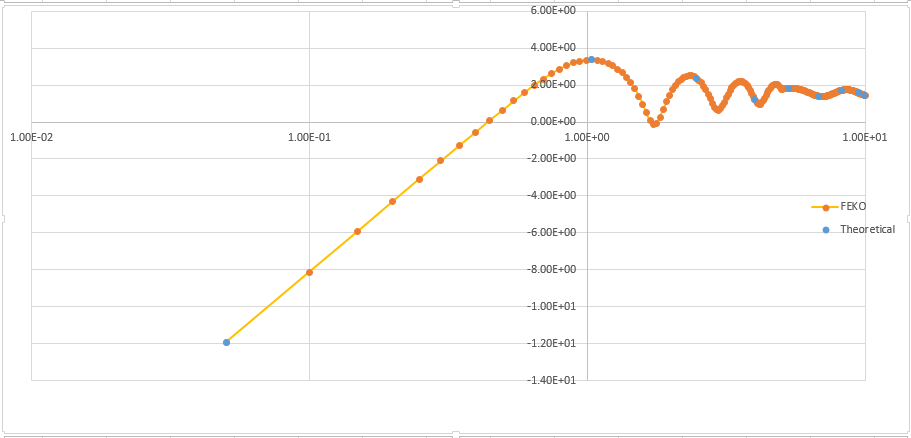
\includegraphics[width = 0.7\textwidth]{backscatter.PNG}
\caption{RCS(dBm2) vs Electrical Circumference}
\end{figure}
\end{frame}

\begin{frame}
\subsection{RCS of sphere with viewing angle}
\frametitle{Simulations in FEKO}
The setup of this problem is that variation of RCS with bistatic angle in both H and E planes is studied and validated against theoretical values.
The setup is as follows:
\begin{itemize}
\item frequency = 70MHz
\item Sphere is a perfect electric conductor
\item Sphere is meshed with 458 triangles.
\end{itemize}
\begin{figure}[H]
\centering
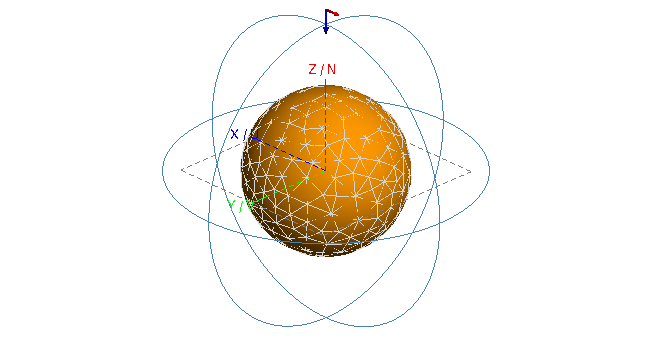
\includegraphics[scale = 0.5]{prob2.PNG}
\end{figure}
\end{frame}

\begin{frame}
\frametitle{Simulations in FEKO}
\begin{figure}[H]
\begin{subfigure}{0.48\textwidth}
\centering
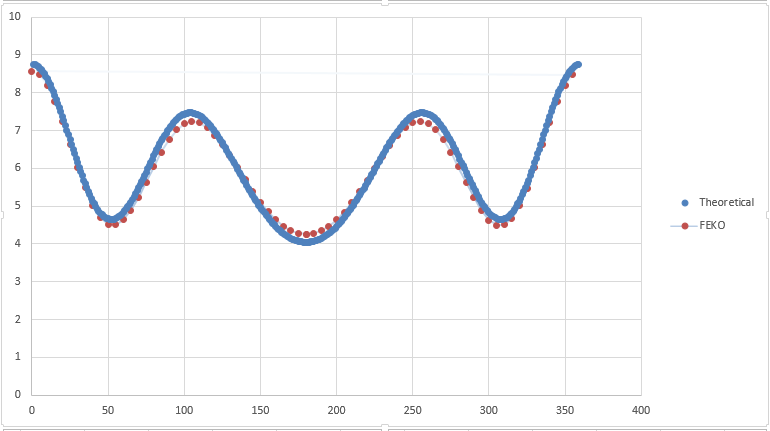
\includegraphics[width = \linewidth]{eplane.PNG}
\caption{RCS vs bistatic angle in E-plane}
\end{subfigure}
\begin{subfigure}{0.48\textwidth}
\centering
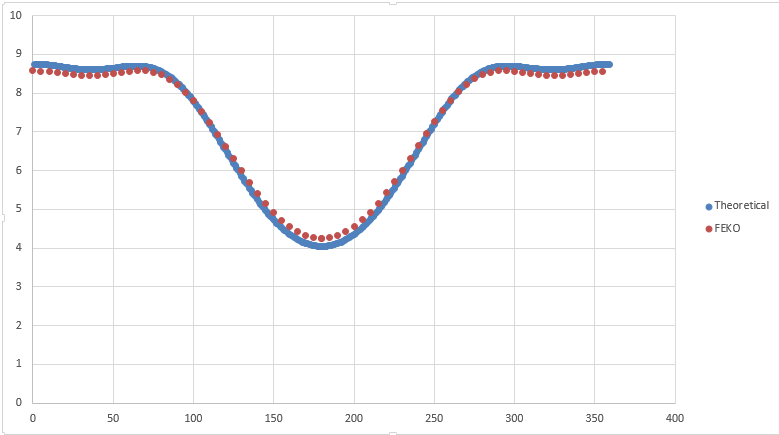
\includegraphics[width = \linewidth]{hplane.PNG}
\caption{RCS vs bistatic angle in H-plane}
\end{subfigure}
\end{figure}
\end{frame}

\begin{frame}
\frametitle{Simulations in FEKO}
\subsection{Sphere coated with dielectric}
The previous two simulations were run for a perfectly electrical conductor sphere. The following simulations now will have a dielectric coating over the sphere  or the sphere itself is made up of a dielectric material.\\ 
Case 1 parameters are :
\begin{itemize}
\item Wavelength = 1 m
\item Core radius = 0.3423 m made up of perfectly conducting sphere
\item Material thickness = 0.1017 m of coating
\item $\epsilon'= 4, \mu' = 1$  
\end{itemize}
This coating has no loss components.
\end{frame}
\begin{frame}
\frametitle{Simulations in FEKO}
\begin{figure}[H]
\centering
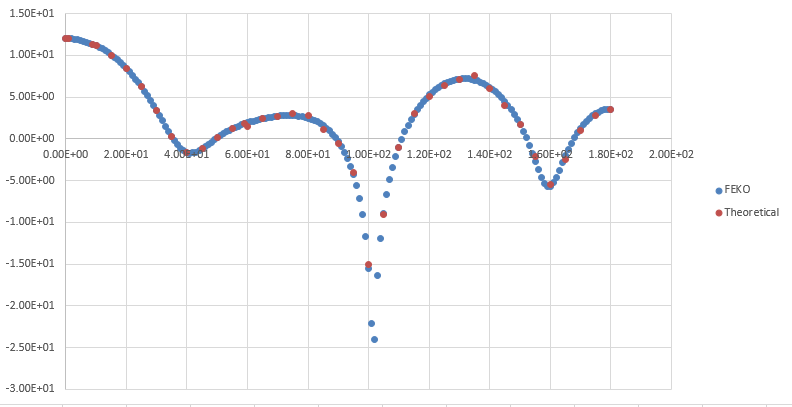
\includegraphics[width = \textwidth]{case1.PNG}
\caption{RCS vs bistatic angle in H-plane}
\end{figure}
\end{frame}
\begin{frame}
\frametitle{Simulations in FEKO}
Case 2 is of a dielectric coating with a loss term in electric permeability. The following are the parameters:
\begin{itemize}
\item Wavelength = 1m
\item Core radius = 0.5 m made up of perfectly conducting sphere
\item Material thickness = 0.1 m of coating
\item $\epsilon' = 4, \epsilon'' = 1, \mu' = 1$
\end{itemize}
This coating has a loss component in electric permeability. There will be losses due to dissipation in electrical field amplitudes. 
\end{frame}
\begin{frame}
\frametitle{Simulations in FEKO}
\begin{figure}[H]
\centering
\begin{subfigure}{0.48\textwidth}
\centering
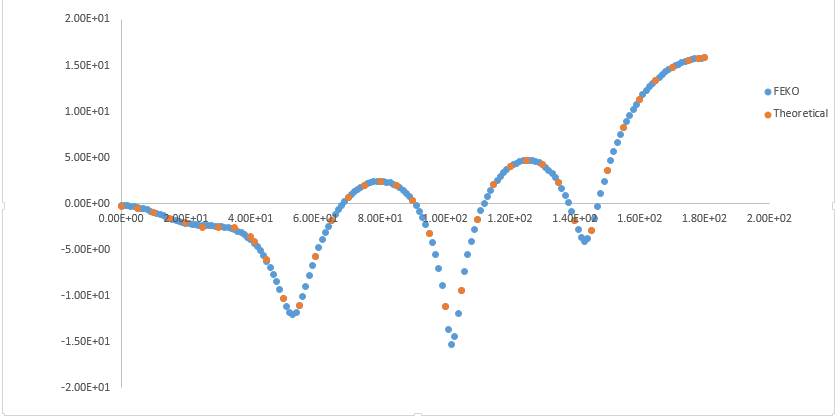
\includegraphics[width = \linewidth]{case2.PNG}
\caption{RCS vs bistatic angle in E-plane}
\end{subfigure}
\begin{subfigure}{0.48\textwidth}
\centering
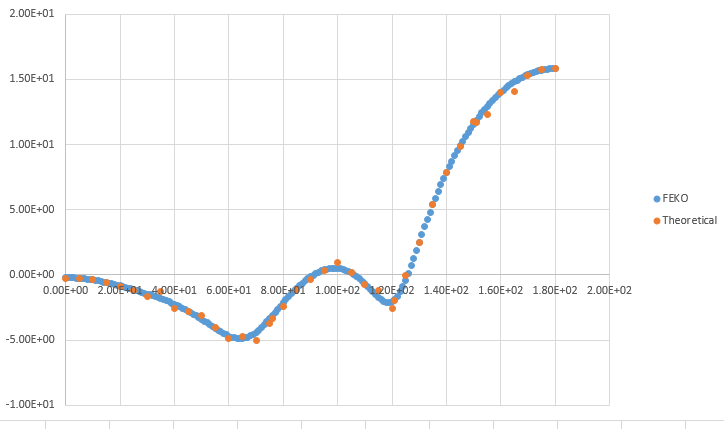
\includegraphics[width = \linewidth]{case2hplane.PNG}
\caption{RCS vs bistatic angle in H-plane}
\end{subfigure}
\end{figure}
\end{frame}
\begin{frame}
\frametitle{Simulations in FEKO}
Case 3 is of a dielectric coating with a loss term in electric permeability. The following are the parameters:
\begin{itemize}
\item Wavelength = 1m
\item Core radius = 0.8 m made up of perfectly conducting sphere
\item Material thickness = 0.2 m of coating
\item $\epsilon' = 1.6, \epsilon'' = 0.8, \mu' = 1$
\end{itemize}
This coating has a loss component in electric permeability. There will be losses due to dissipation in electrical field amplitudes. 
\end{frame}

\begin{frame}
\frametitle{Simulations in FEKO}
\begin{figure}[H]
\centering
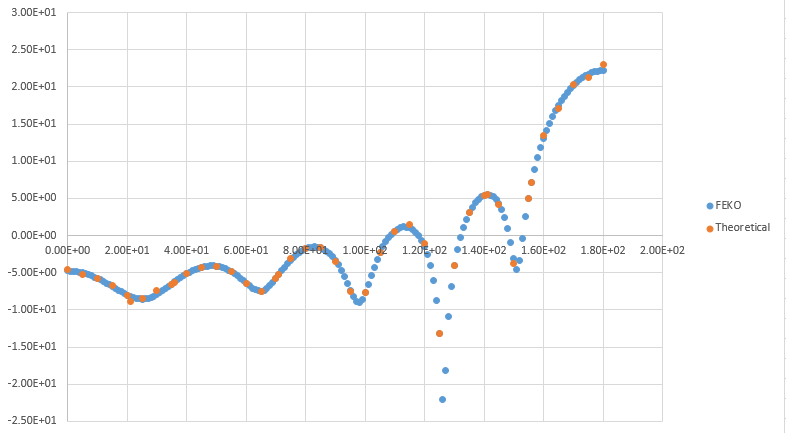
\includegraphics[width = \textwidth]{coating3.PNG}
\caption{RCS vs bistatic angle}
\end{figure}
\end{frame}

\begin{frame}
\frametitle{Simulations in FEKO}
\subsection{Dielectric Sphere}
Case 4 is of a dielectric sphere with no loss terms. The following are the parameters:
\begin{itemize}
\item Wavelength = 1m
\item Core radius = 0.5 m made up of dielectric sphere
\item $\epsilon' = 4, \mu' = 1$
\end{itemize}
\end{frame}
\begin{frame}
\frametitle{Simulations in FEKO}
\begin{figure}[H]
\centering
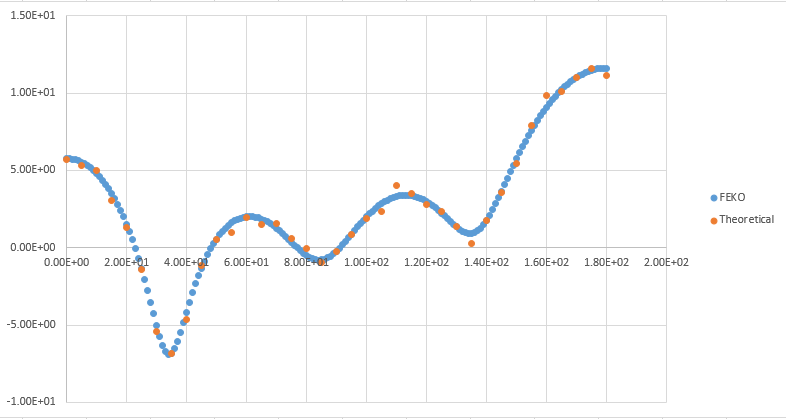
\includegraphics[width = \textwidth]{case4.PNG}
\caption{RCS vs bistatic angle}
\end{figure}
\end{frame}

\begin{frame}
\frametitle{Simulations in FEKO}
Case 5 is of a dielectric sphere with loss terms in both electrical and magnetic permeability. The following are the parameters:
\begin{itemize}
\item Wavelength = 1m
\item Core radius = 1 m made up of lossy dielectric sphere
\item $\epsilon' = 1.6, \epsilon'' =0.8, \mu' = 0.8, \mu''=0.2$
\end{itemize}
This material has both magnetic and electrical losses causing the loss in amplitude of both the fields.
\end{frame}
\begin{frame}
\frametitle{Simulations in FEKO}
\begin{figure}[H]
\centering
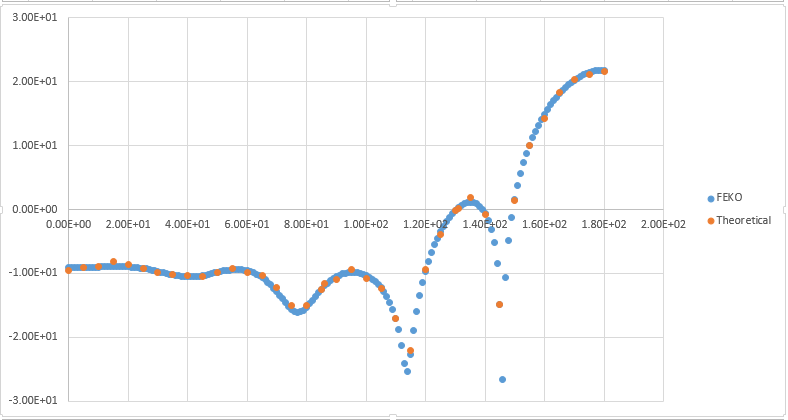
\includegraphics[width = \textwidth]{case5.PNG}
\caption{RCS vs bistatic angle}
\end{figure}
\end{frame}
%------------------------------------------------

\begin{frame}
\section{References}
\frametitle{References}
\footnotesize{
\begin{thebibliography}{99} % Beamer does not support BibTeX so references must be inserted manually as below
\bibitem{p1} Eugene F. Knott-Radar Cross Section-SciTech Publishing (2006)
\bibitem{p1} UserManual new for FEKO
\bibitem{p1} ExampleGuide 7.0 for FEKO
\bibitem{p1} Code Development for Radar Absorbing Materials.
\end{thebibliography}
}
\end{frame}

\begin{frame}
 \section{Future Work}
 \frametitle{Future Work}
 In the future, as a continuation to this project, RCS analysis of complex Aerospace shapes are to be done for different frequencies and specular angles to optimize the Radar Cross sections. \\
 It is also hoped that RCS analysis to be coupled with CFD analysis iteratively to check the effect of efficiency of one on another which will be helpful in shape optimization techniques of Aerospace shapes.
\end{frame}


%------------------------------------------------

\begin{frame}
\Huge{\centerline{Thank You}}
\end{frame}

%----------------------------------------------------------------------------------------

\end{document}